\section{Evaluation}\label{experiment}

In this section, we evaluate the performance improvements brought by TAFL using well-known benchmarks. The evaluation setup environments are firstly described, including the used benchmarks, evaluation tools, experimental infrastructure and research questions we are trying to answer. We also represent and explain our evaluation results.

\subsection{Evaluation Setup}

\begin{table*}[t]
\centering
% \begin{adjustbox}{max width=\columnwidth}
\begin{adjustbox}{max width=\textwidth}

\begin{tabular}{|l|l|l|l|l|l|l|l|l|l|l|l|l|l|l|l|}
\hline
\multirow{2}{*}{\textbf{App}} & \multicolumn{3}{l|}{\textbf{AFL}} & \multicolumn{3}{l|}{\begin{tabular}[c]{@{}l@{}}\textbf{TAFL-sen}\end{tabular}} & \multicolumn{3}{l|}{\begin{tabular}[c]{@{}l@{}}\textbf{TAFL-com}\end{tabular}} & \multicolumn{3}{l|}{\begin{tabular}[c]{@{}l@{}}\textbf{TAFL-deep}\end{tabular}} & \multicolumn{3}{l|}{\begin{tabular}[c]{@{}l@{}}\textbf{TAFL-rare}\end{tabular}} \\ \cline{2-16} 
                     &\textbf{ first(min) }  & \textbf{crash}  & \textbf{path}  & \textbf{first(min)}                   & \textbf{crash}                  &\textbf{ path }                 & \textbf{first(min)}                 & \textbf{crash                 } &\textbf{ path    }              & \textbf{first(min) }                  & \textbf{crash}                & \textbf{path}             &\textbf{ first(min)}                  & \textbf{crash}                  & \textbf{path}                  \\ \hline
base64         &   23.15  &             53              &        155              &        -34.64\%            &         +30.18\%          &         -15.48\%               &      -38.83\%              &     +28.30\%                  & -4.51\%  &          -92.74\%           &      +15\%               &       -2.5\%               & -16\%& +66\% & +87.4\% \\ \hline
md5sum             &   1.95      &    32    &  370     &       -18.22\%                  &     +21.87\%                   &  +2.43\%       &       -35.44\%     &       -12.5\%        &      -2.43\%      &        -52.91\%     &         +31.25\%   &                      +4.32\% &        -28.86\%     &          +15.62\%      &      +5.13\%      \\ \hline
uniq                    &   1072.65     &   1    &   126 &       -29.95\%            &          0\%          &     0\%                &       -7.07\%               &     0\%               &     +1.28\%                  &      -84.81\%                 &    0\%                 &       +4.76\%             &   -13.51\%       &        0\%               &     +6.34\%     \\ \hline
who                     &   937.31   &     2  &   202        &           -6.18           &       0\%           &     +7.9\%                &    -29.66\%              &       0\%            &       -7.4\%                 &          -15.37\%            &      0\%              &                     +10.89\% & +4.36\%       &   0\%    & +1.98\%            \\ \hline
libxml2-2.9.2     &   534.61      &    12    &   6080    &        -60.84\%              &     +41.66\%               &       +5.50\%                &       +20.54\%                &       -33.33\%       &+3.79\%  &     -35.90\%    &        +133.33\%  &      +7.36\%            &      -56.82\%          &         +216.66\%            &      +12.61\%                            \\ \hline
libtiff-3.7.0        &   0.08          &    52    &  469       &         0\%                  &      +21.53\%                 &       +15.35\%                &        0\%                         &     +17.30\%                  &     +10.87\%                 &          0\% &       +36.53\%   &        +11.08\%             &         0\%               &         +23.07\%              &    +15.99\%                  \\ \hline
%libtasn1-4.12      &    1318.53     &    1    &    776   &          -             &        -                &        -4.25\%               &        -                 &          -              &          -1.28\%             &        -                 &        -                &      +1.15\%                 &            -             &           -              &        +4.89\%               \\ \hline
bison-3.0.4        &  52.14       &   161     &   3591    &           -95.43\%              &       +18.01\%                 &      +8.71\%               &     -90.64\%               &    +4.96\%      & +4.42\%           &     -58.38\%        &          +31.67\%           &         +3.70\%               &     -72.13\%                &        +19.87\%              &        +29.15\%                        \\ \hline
cflow-1.5            &     22.65    &    166    &           1331                    &   -68.78\%                  &    +6.02\%                  &     -0.52\%                   &       -55.05\%              &        +44.57\%        &    +2.55\%                   &    +51.74\% &        -3.61\%             &        -0.75\%                 &         -58.41\%               &     +5.42\%      &    +0.75\%      \\ \hline
libjpeg-tubo-1.2.0   &  117.25      &   22     &   2908    &        -18.43\%         &      -18.18\%                  &      -3.25\%                 &       -53.72\%    &     +104.54\%       &         +8.70\%        &       -108.31\%                  &                       -18.18\% &         -10.24\%              &      +10.53\%                   &     -45.45\%                    &     -3.12\%                  \\ \hline
%jasper-2.0.14     &   3.45      &   283     &       &                         &                        &                       &                         &                        &                       &                         &                        &                       &                         &                         &                       \\ \hline
%ImageMagick-7.0.8    &         &        &       &                         &                        &                       &                         &                        &                       &                         &                        &                       &                         &                         &                       \\ \hline
\textbf{Average}         &     -      &   -   &  -  &\textbf{-36.94\%} & \textbf{+15.05\%} & \textbf{+2.29\% }    & \textbf{-32.21\% }& \textbf{+17.09\%} & \textbf{+1.91\%} & \textbf{-20.01\%} & \textbf{+25.12\% }& \textbf{+3.17\%} & \textbf{-28.27\%} & \textbf{+31.26\%} & \textbf{+17.39\%}  \\\hline 
\end{tabular}
\end{adjustbox}
\caption{Results of Directing Towards Four Kinds of Promising Regions}
\label{TargetAreas}
\end{table*}


\textbf{Evaluation Datasets}: A widely used benchmark (i.e., LAVA-M ) and some popular open source projects are selected for the evaluation. The programs in selected benchmarks are known to have specific vulnerabilities, and hence form a ground-truth corpus for evaluating fuzzing tools.
\begin{itemize}

   \item \textbf{LAVA-M Dataset}. LAVA-M consists of four buggy versions of Linux utilities, i.e., \texttt{base64}, \texttt{md5sum}, \texttt{uniq} and \texttt{who}. It was generated by automatically injecting known vulnerabilities into hard-to-reach regions of the source code \cite{lava}. It is commonly used as a benchmark for evaluating the capability of various fuzzing tools. The authors of recent fuzzing tools (e.g. VUzzer\cite{rawat2017vuzzer}, CollAFL\cite{gancollafl}, and Angora \cite{chen2018angora} all used this benchmark.
        
    \item \textbf{Real-World Projects}. Some popular open source Linux projects are selected, including document process libraries (e.g., libxml2), image processing libraries (e.g., libtiff) and so on. They are chosen based on the following criteria: popularity in the community, development activeness, and diversity of categories.  
\end{itemize}


\textbf{Evaluation Tools}: AFL based greybox fuzzing is our focus. Thus AFL and its variants based on source level instrumentation are our comparison targets.  Furthermore, we only select tools that are available for download online. These tools include:
    
\begin{itemize}

    \item \textbf{AFL-2.52b}:  It is the latest version of official AFL.
    
    \item \textbf{AFLFast}: It is an AFL variant that tries to balance the energy distribution by spending more energy on low-frequency path.
    
    \item \textbf{FairFuzz}: It is an AFL variant that guides the fuzzer to approach rarely reached branches.
    
    \item \textbf{TAFL}: It is our extension of AFL, which is integrated with improvements of directing towards four kinds of promising vulnerable regions and granularity-aware scheduling of different kinds of mutation operators. 
\end{itemize}


\textbf{Experimental Infrastructure}: Fuzzing tools are evaluated on collected benchmarks with the same configuration, i.e., a virtual machine configured eight core of 2GHz Intel CPU and 8 GB RAM, running Ubuntu 16.04.


\textbf{Research Questions}: We evaluated each improvement and integrated performance of TAFL, and try to answer the following research questions:

\begin{itemize}

    \item \textbf{RQ1:} The effectiveness of directing towards four kinds of vulnerability promising areas.
    
    \item \textbf{RQ2:} The effectiveness of scheduling of different mutation operators.
    
    \item \textbf{RQ3:} The performance of integrated TAFL compared with existing mainstream AFL based greybox fuzzers.
    
\end{itemize}



\subsection{Evaluation of Directing Towards Promising Regions}
\label{sec:directing}
The effectiveness of directing fuzzers toward four kinds of promising regions that are more likely for a vulnerability to reside are evaluated. Furthermore, we compare the results with the  original AFL. Note that TAFL used in this evaluation is only integrated with improvement of guidance, without scheduling of mutators. Each project is executed ten times for 24 hours in order to reduce the random noise of fuzzing. Results are collected and illustrated in Table \ref{TargetAreas}. 
In the table, the four directed fuzzing strategies are donated as \textit{TAFL-sen} (sensitive region),  \textit{TAFL-com} (complex region), \textit{TAFL-deep}  (deep region) and \textit{TAFL-rare}  (rare-reach region) respectively.
Three measurement metrics, including time to trigger the first crash, total unique crashes and total paths are used. They are labeled as \textit{first}, \textit{crash} and \textit{path} respectively in the table.
 % are used to show the effectiveness and performance of four kinds of promising vulnerable regions guided search strategies.
\subsubsection{First Blood }

Time to trigger the first crash is an important factor to evaluate a directed fuzzing tool. As we could see from Table \ref{TargetAreas}, all the four directed fuzzing strategies advance the time to find the first crash in most cases. The average advance ratio for detecting first blood are 36.94\%, 32.21\%, 20.91\%, 28.27\% for four kinds of area directed strategies respectively. Generally speaking, sensitive regions guided fuzzing has better performance of triggering the first crash on selected benchmarks. In some specific cases like bison-3.0.4, sensitive area directed strategy brings 95.43\% performance improvement. This result proves that if a code region contains more memory and string related instruments, it has more chances to occur memory corruption problems.

\subsubsection{Unique Crashes}
Another important characteristic of a good fuzzers is its ability to find unique crashes in limited time. Although the same root crash may cause multiple unique crashes, and some are even not exploitable, in general, more unique crashes indicate better chances to find vulnerabilities. 
% In AFL, different paths to the same crash point are marked as separate unique crashes. Thus unique crashes metric also show the explored degree of vulnerable point. The total crashes could indirectly prove effectiveness of improvement of guidance. 
As can be seen from Table \ref{TargetAreas}, four regions directed strategies get more unique crashes in most cases, and average improvements are 15.05\%, 17.09\%, 25.12\%, 31.26\% respectively. The results prove the effectiveness of improvement in directing fuzzing toward promising areas. Moreover, among four kinds of region directed strategies, rare-reach region directed strategy performs the best in general. Especially, its improvement reaches 216.66\% in the case of libxml2-2.9.2. It proves that regions without sufficient testing may have higher probabilities for a vulnerability to reside.

\subsubsection{Total Paths}
Another important factor is the number of total paths a fuzzer can traverse in limited time. For four vulnerable region directed strategies, the average improvements are 2.29\%, 1.91\%, 3.17\% and 17.39\% respectively. The result shows that rarely reachable region guided strategy is much more helpful to path growth. Furthermore, we could conclude from the above results that the strategy of directing fuzzing towards rarely reachable regions outperform all the other on selected benchmarks.



\subsection{Evaluation of Scheduling of Different Mutators}
Code coverage is one of the critical factors for fuzzers' success. 
% It is also the most important metric to show performance of different distribution strategies of various mutation operators. 
We use two coverage related metrics (i.e., path growth over time and total reachable paths) to validate the effectiveness of our improvement to mutator scheduling. The evaluation was performed on collected benchmarks, and each project ran ten times for 24 hours for the sake of reducing fuzzing's random noise. The result is counted and illustrated in Table \ref{EffectiveOfMutatorDistribution}.

\subsubsection{Path Growth Over Time}
Path growth over time is a direct indicator of fuzzer's ability to explore new paths. The original AFL and AFLFast are modified to add improvement of scheduling for different mutation operators. Due to limited space of the article, we selected partial results to illustrate the effectiveness of scheduling of mutation operators in Fig. \ref{mutateSchedule}. For more empirical results, please refer to our website (\url{https://sites.google.com/view/tafl}).

\begin{figure}[t]
    \centering
    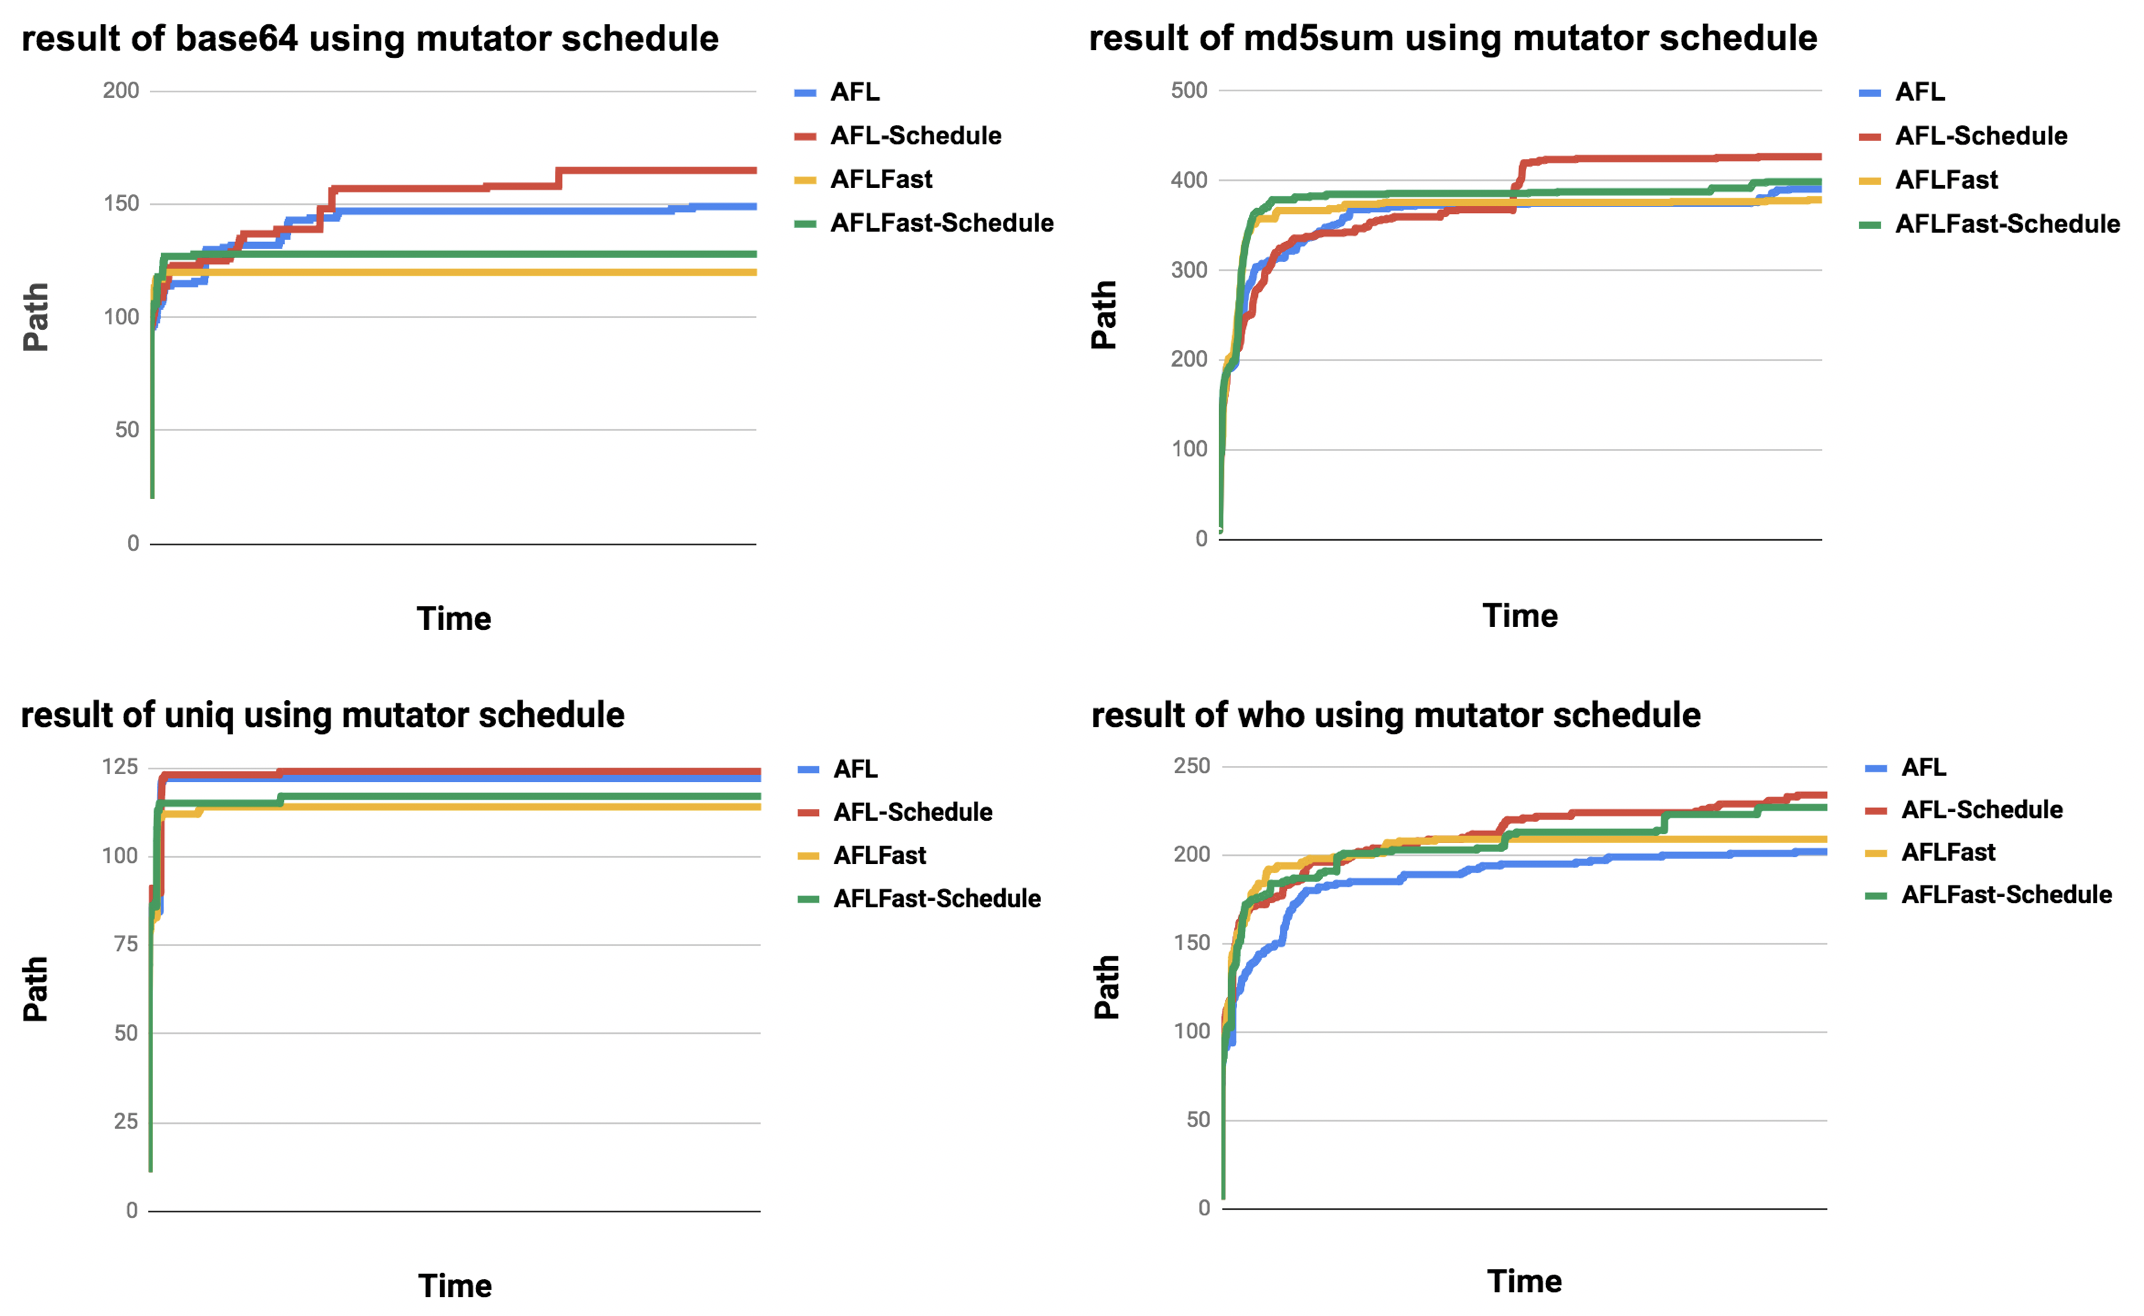
\includegraphics[width=\columnwidth]{pic/scheduleLAVM12.png}
    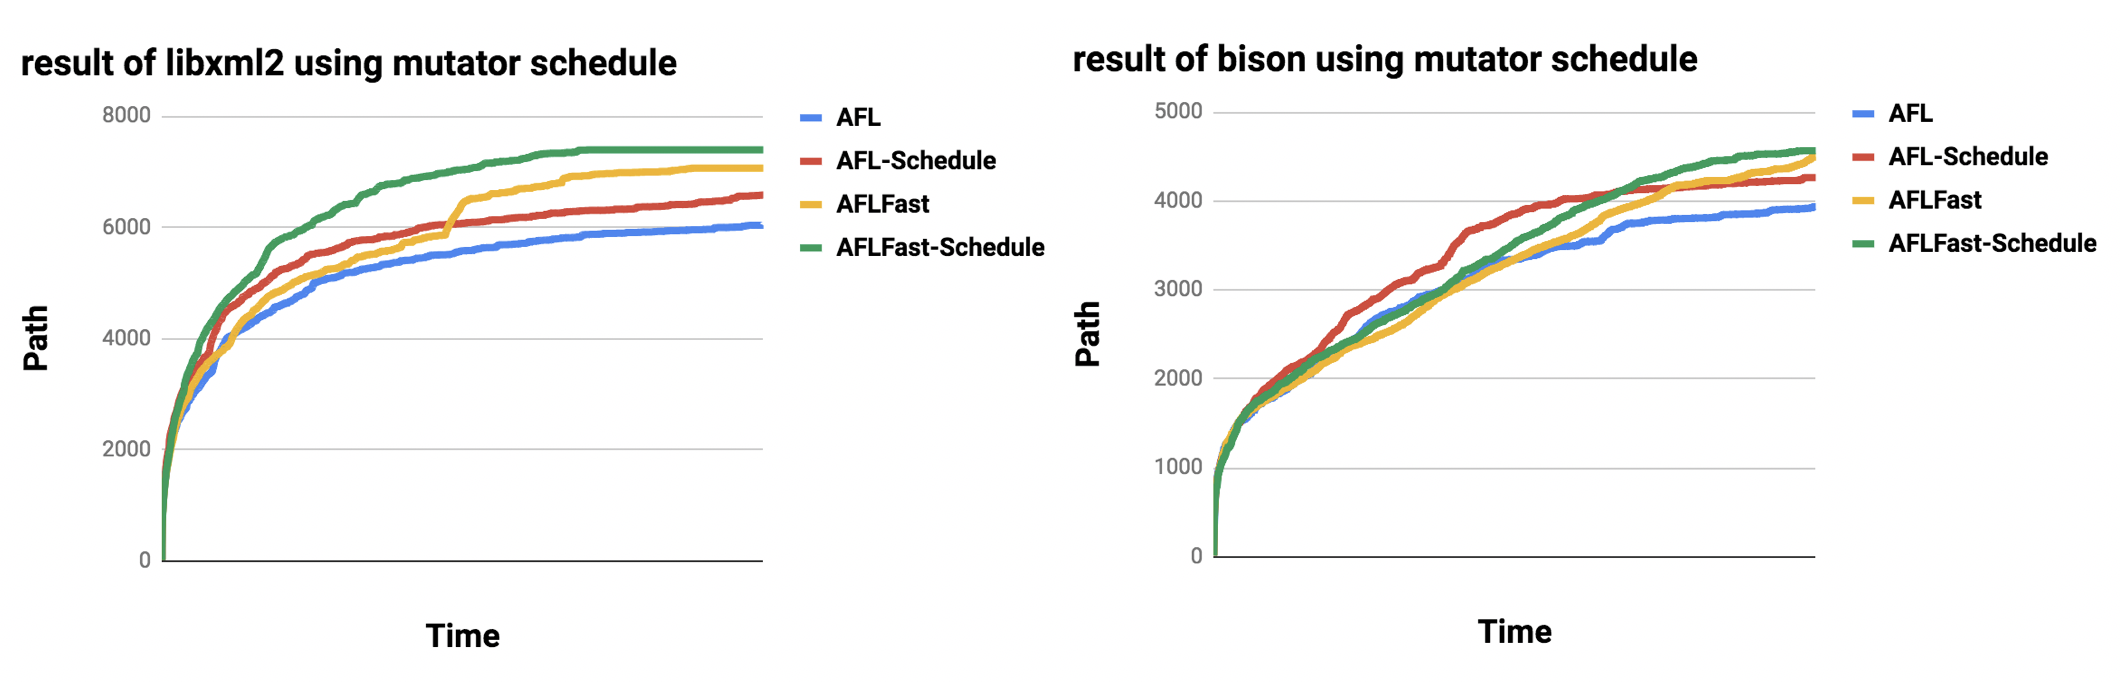
\includegraphics[width=\columnwidth]{pic/schedule22.png}
    \caption{Results of Scheduling Mutators}
    \label{mutateSchedule}
\end{figure}

As can be seen from above Fig.\ref{mutateSchedule}, fuzzers with scheduling of mutators could trigger new paths more quickly than than those without scheduling in most cases. Scheduling of mutators is helpful to maximize code coverage in limited time. The results prove the effectiveness of scheduling mutators. Besides, we observe that AFLFast is better than AFL in most cases within 24 hours. However, in some case such as base64, AFLFast's performance is worse than AFL. In practice, AFLFast's will slow down to zero after a specific time. The reason is that low-frequency paths in base64 are time-consuming, which stuck AFLFast.

\subsubsection{Improvement of Total Path}

\begin{table}[t]
\centering
\begin{adjustbox}{max width=\columnwidth}
\begin{tabular}{|l|l|l|l|l|}
\hline
\textbf{Application }      & \textbf{AFL} & \textbf{AFL-schedule} & \textbf{AFLFast} & \textbf{AFLFast-Schedule} \\\hline
base64            &   155 &  +10.7\%     &    120     &    +6.6\%              \\ \hline
md5sum          &   370 &    +5.2\%    &      378   &      +8.9\%            \\ \hline
uniq                 &  126   &   +3.2\%     &   114      &     +2.6\%              \\ \hline
who                  &  201   &  +15.8\%      &   219      &    +8.6\%            \\ \hline
libxml2-2.9.2   & 6080   &   +14.7\%      &  6402       & +13.9\%        \\ \hline
libtiff-3.7.0       &  469   &   -0.9\%     &      514   &       +2.5\%          \\ \hline
bison-3.0.4       &  3591   &      +9.4\%        &   4324      &   +4.7\%      \\ \hline
cflow-1.5           & 1331    &   +1.6\%     &   1294      &  +2.7\%               \\ \hline
libjpeg-tubo-1.52 & 2908    &    +3.6\%    &   3087      &   +1.3\%         \\ \hline
\textbf{Average}               &   -  &   \textbf{+7.03\%}    &    -      &     \textbf{+4.82\% }                \\ \hline
\end{tabular}
\end{adjustbox}
\caption{Paths Improvement of Scheduling Mutators}
\label{EffectiveOfMutatorDistribution}
\end{table}


Furthermore, we show the total executed paths by AFL, AFLFast and their improved versions in Table \ref{EffectiveOfMutatorDistribution}.
Scheduling of mutators is useful to improve code coverage in most cases. For AFL and AFLast, the average increased percentage on selected benchmarks are 7.03\% and 4.82\% respectively. In certain cases such as libxml2-2.9.2, the promotion percentage could be as high as 15.8\% and 14.7\%. In some lousy cases such as libtiff-3.7.0, the ratio could drop to -0.9\%. We observe that the the difference of different fuzzing strategies' efficiency are obvious when limited time is given. If enough time is given, the eventual discovered paths will be very close for different fuzzing strategies. This is because all the easily reachable regions are already explored.

\subsection{Evaluation of Integrated Performance}
In this section, we evaluate the overall performance of TAFL compared with AFL, AFLFast and FairFuzz, which means TAFL is integrated with the capability to direct towards promising regions and
to schedule of different mutators. Similar to Section~\ref{sec:directing}, the same set of metrics are used to measure the performance. Each project is fuzzed ten times for 24 hours in order to reduce the random noise of fuzzing, and the results are collected and illustrated in Table \ref{Integration}.


\begin{table*}[t]
\centering
% \begin{adjustbox}{max width=\columnwidth}
\begin{adjustbox}{max width=\textwidth}
\begin{tabular}{|l|l|l|l|l|l|l|l|l|l|l|l|l|}
\hline
\multirow{2}{*}{\textbf{App}} & \multicolumn{3}{l|}{\textbf{AFL}} & \multicolumn{3}{l|}{\textbf{AFLFast}} & \multicolumn{3}{l|}{\textbf{FairFuzz}} & \multicolumn{3}{l|}{\begin{tabular}[c]{@{}l@{}}\textbf{TAFL-rare}\end{tabular}} \\ \cline{2-13} 
                             &\textbf{ first  blood   }        &\textbf{ crashes }    &  \textbf{paths}     &\textbf{ first blood  }          & \textbf{crashes }   & \textbf{paths }     &\textbf{ first  blood  }     &  \textbf{crashes }   & \textbf{ paths }       &\textbf{ first blood }              &\textbf{ crashes }        &\textbf{ paths }                              \\ \hline
base64               &  23.15          &    53       & 155     &     59.46     &    52       &   139        &   0           &      0       &    134     &      20.3          &       83          &         288                          \\ \hline
md5sum            &    3.95           &    32       & 370    &    2.13         &    37       &    378       &   5.81      &    30       &     301    &      3.23           &       43          &        412                         \\ \hline
uniq                   &    1072.65     &   1           & 126    &    901.01     &    1          &  132          &  0            &     0        &    134     &      717.19        &       1             &        144                          \\ \hline
who                   &    937.31       &    2          & 202   &  890.33      &    2          &  209         &  0            &     0        &     206    &     915.54      &       2             &         216                         \\ \hline
libxml2-2.9.2    &   534.61        &    12    &  6080   &    560.23     &     17       &  6402       &  826.7    &     22      &   6410    &     330.81       &      41            &        7331                        \\ \hline
libtiff-3.7.0       &     0.08          &   52    &    469   &      0.08        &   52        &    512         &  0.08      &     62    &   490       &     0.08           &      68            &       571                         \\ \hline
%libtasn1-4.12    &    1318.53      &    1      &    776   &                      &               &                &                 &              &                 &                                  &                    -       &                                          \\ \hline
bison-3.0.4      &   52.14            &    161 &   3591  &    42.23        &  208       &   4324    &    5.68     &  119       &  3214       &     19.53          &    196           &        4709                        \\ \hline
cflow-1.5          &   22.65           &    166  &   1331   &    5.81        &      177    &    1321    &     33.52   &    204   &   1197        &     7.42            &    173           &        1412                         \\ \hline
libjpeg-tubo-1.2.0   &   117.25   &    22    &   2908    &   58.5       &      12    &    3087    &   786.03   &    4      &    1681       &     85.91          &    12             &        2978                       \\ \hline
%jasper-2.0.14        &         &        &       &          &          &        &          &          &         &                         &                        &                       &                         &                        &                       &                         &                        &                       &                         &                         &                       \\ \hline
%ImageMagick-7.0.8    &         &        &       &          &          &        &          &          &         &                         &                        &                       &                         &                        &                       &                         &                        &                       &                         &                         &                       \\ \hline
Average  &    337.08           &     55.66      &    1692.44       &      279.97             &    62         &   1833.77            &      276.34       &    49      &    1529.66           &     248.18        &      68.77          &         2006.78 \\ \hline
\textbf{Improvement}  &    -                     &     -               &    -                   &    \textbf{ -16.94\% }           &\textbf{+11.39\%  }         &  \textbf{ +8.35\% }         &    \textbf{  -18.01\%}       &    \textbf{-11.97\%}        &    \textbf{-9.62\%}            &  \textbf{-26.37\%}      &   \textbf{+23.55\% }    &  \textbf{+18.57\% }             \\ \hline
\end{tabular}
\end{adjustbox}
\caption{Comparison Results of TAFL and AFL based Greybox Fuzzers}
\label{Integration}
\end{table*}

\subsubsection{First Blood}
As is shown in Table \ref{Integration}, the integration of improvements is effective to advance the time to trigger the first crash. In general, the time to trigger the first crash is advanced 26.37\% after using mutator schedule. This is better than AFLFast and FairFuzz.% In general, the time to trigger the first crash is advanced by 26.37\% in TAFL after using mutator schedule.

\subsubsection{Unique Crashes}
As can be seen from the Table \ref{Integration}, compared to AFL and its extension AFLFast, TAFL-rare detects more crashes within 24 hours on selected benchmark. The improvements in total crashes of AFLFast and TAFL- rare are 11.39\% and 23.55\%. TAFL-rare is twice as many as AFLFast. Meanwhile, FairFuzz performs poor, especially on LAVA-M benchmark, it cannot detect crashes in base64, uniq, and who programs, but it could get a better result on the cflow-1.5 project.
%TAFL-rare detects more crashes within 24 hours on selected benchmark. The improvements to AFLFast and TAFL-rare are 11.39\% and 23.55\% respectively. Meanwhile, FairFuzz performs poorly, especially on LAVA-M benchmark. It cannot detect crashes in \texttt{base64}, \texttt{uniq}, and \texttt{who} programs, but it could get a better result on the cflow-1.5 project. 

\subsubsection{Total Paths}
As can be seen from the Table \ref{Integration}, the promising regions directed and mutator schedule strategy are helpful to improvement on the entire path. On the selected benchmarks, TAFL-rare brings an average improvement of 18.57\%, while the average improvements to AFLFast and FairFuzz are 8.35\% and -9.62\% respectively. Furthermore, TAFL helps us find five unknown bugs and identify one new CVE\cite{bugs}. 
%The combination of the two strategies is helpful to the improvement on the entire path. On the selected benchmarks, TAFL-rare brings an average improvement of 18.57\%, while the average improvements to AFLFast and FairFuzz are 8.35\% and -9.62\% respectively. Furthermore, TAFL helps us find five unknown bugs and identify one new CVE\cite{bugs}. 
